\chapter{Descripción del problema}\label{chapter:problemIntro}

Dado un conjunto de puntos de la forma $<ti, yi>$ se desea determinar automáticamente el sistema de ecuaciones diferenciales ordinarias que mejor describe el conjunto de datos y que además, sea lineal en los parámetros.

A continuación se describirá brevemente qué significa que la ecuación diferencial sea lineal en los parámetros y que mejor describa los datos.

\section{Función lineal con respecto a los parámetros}

Que el sistema sea lineal en los parámetros significa que cada componente de la parte derecha de la ecuación diferencial es una función de la forma:

$$f_j(t,y) = a1 * g1(t,y) + a2 * g2(t,y) + …  + an * gn(t,y)$$

donde los ai son parámetros y todas las funciones gi(t,y) son funciones que dependen de la variable t, de la variable y, pero no dependen de ningún parámetro.  Un ejemplo de sistema que cumple esta características es el sistema SIR:

$$S’ = - a*I*S$$
$$I’ = a*I*S - b*I$$
$$R’ = b*I$$

Este modelo indica la cantidad de individuos susceptibles, infectados y recuperados de una enfermedad en un instante de tiempo. En este caso, se tiene que la función

$$f_S (t,S,I,R) = a1 * g_s1 (t,S,I,R)$$

donde:

$$g_s1(t,S,I,R) = -I*S$$

La parte de derecha de la segunda ecuación (I’ = a\*I\*S - b*I) sería:

$$f_I (t,S,I,R) = b1 * g_I1 (t,S,I,R) + b2 * g_I2 (t,S,I,R)$$

donde:

$$g_I1(t,S,I,R) = I*S, y g_I2(t,S,I,R) = -I$$

La parte de derecha de la tercera ecuación $(R’ = b*I)$ sería:

$$f_R (t,S,I,R) = b1 * g_R1 (t,S,I,R)$$

donde:

$$g_R1(t,S,I,R) = I$$

En este caso, se cumple además, que algunos de los parámetros presentes en varias de las ecuaciones son los mismos, pero eso no es un requisito para que sea lineal con respecto a las parámetros.

Este sistema SIR se puede ver gráficamente como:

\begin{figure}[!h]
    \centering

    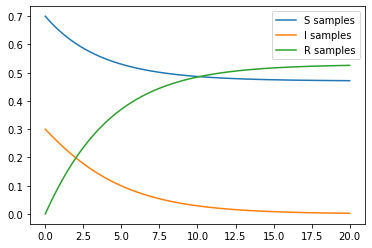
\includegraphics[width=3in]{Graphics/sir_model.png}

    \caption{ \small{Modelo de SIR.}}

    \label{sir_model}

\end{figure}

y este indica en una población con una enfermedad, como se va desplazando la cantidad de susceptibles, infectados y recuperados a lo largo del tiempo.

\section{Sistema de ecuaciones diferenciales que mejor describa los datos}

Dado un conjunto de puntos de la forma $<ti, yi>$ y un sistema de ecuaciones diferenciales $y’ = f(t,y)$, se puede tener un indicador de cuán bien ese sistema describe esos datos.

Si decimos que $y(ti)$ es la solución de la ecuación diferencial evaluada en el punto $ti$, entonces un indicador de cuán bien ese sistema describe los datos pudiera ser el valor $L$:

$$L = (y(t1) - y1)^2 + (y(t2) - y2)^2 + …  + (y(tn) - yn)^2$$

Esto es una suma de cuadrados, que se puede escribir con una sumatoria, aunque se expresa la versión explícita.

Cuando se usa un valor como L en el que se considera la suma de cuadrados de las diferencias, se dice que estamos en presencia de un problema de mínimos cuadrados, porque lo que se quiere es minimizar esa suma de cuadrados.

Entonces, buscar el sistema de ecuaciones diferenciales que mejor describe los datos, se reduce a buscar el sistema de ecuaciones diferenciales que haga que el valor de L (la suma de cuadrados) sea lo más pequeño posible.

Pero, aquí no interesa cualquier sistema de ecuaciones diferenciales: interesa los que sean lineales con respecto a los parámetros

Este sistema de ecuaciones diferenciales deseado se vería gráficamente como un sistema que solapa al original:

\begin{figure}[!h]
    \centering

    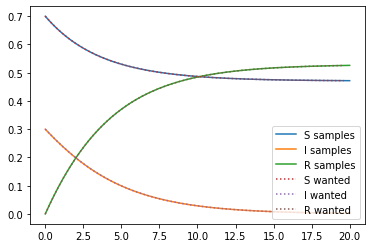
\includegraphics[width=3in]{Graphics/sir_model_wanted.png}

    \caption{ \small{Modelo de SIR original y modelo de SIR que se desea encontrar.}}

    \label{sir_model_wanted}

\end{figure}